\documentclass[a4paper,11pt]{ltjsarticle}
\usepackage{graphicx}
\usepackage{luatexja-fontspec}
\usepackage{caption}
\usepackage{amsmath,amssymb,bm,braket}
\usepackage[english]{babel}
\usepackage{multicol}
\usepackage{titlesec}
%\usepackage{gnuplot-lua-tikz}
\usepackage[top=20truemm,bottom=20truemm,left=20truemm,right=20truemm]{geometry}
\usepackage{array}
\usepackage{upgreek}
\usepackage{fancyhdr}
\renewcommand{\refname}{}
\usepackage{listings,jvlisting}
\usepackage{tikz}
\usepackage[thmmarks,amsmath]{ntheorem}
\usepackage[version=3]{mhchem}
\usetikzlibrary{external}
\tikzexternalize
\lstset{
  basicstyle={\ttfamily},
  identifierstyle={\small},
  commentstyle={\smallitshape},
  keywordstyle={\small\bfseries},
  ndkeywordstyle={\small},
  stringstyle={\small\ttfamily},
  frame={tb},
  breaklines=true,
  columns=[l]{fullflexible},
  numbers=left,
  xrightmargin=0pt,
  xleftmargin=3pt,
  numberstyle={\scriptsize},
  stepnumber=1,
  numbersep=1pt,
  lineskip=-0.5ex
}
\captionsetup[figure]{format=plain, labelformat=simple, labelsep=quad,labelfont=bf,name={Fig.}}
\captionsetup[table]{format=plain, labelformat=simple, labelsep=quad,labelfont=bf}
\parindent = 0pt
%[BoldFont=HGSMinchoE]{MSMincho}[BoldFont=HiraMinProN-W6]{HiraMinPro-W3}
\titleformat{\section}{\normalfont\fontsize{9}{10}\bfseries\fontspec{Times New Roman}}{\thesection.}{1em}{}
\usepackage[backend=biber,sorting=none,style=numeric,maxnames=99,minnames=1]{biblatex}
\addbibresource{utility/REFERENCES.bib}
\defbibheading{bibliography}[\refname]{%
  \section*{REFERENCES}%
  \vspace{-7pt}  % ここで空白を調整。お好みの値に変更してください。
}
\newfontfamily\subsectionfont{Times New Roman} % サブセクション用フォント
\titleformat{\subsection}
  {\normalfont\large\bfseries} % サブセクションのフォントを指定
  {\thesubsection}{1em}{}
\renewbibmacro{in:}{}
\renewbibmacro*{journal+issuetitle}{%
  \addcomma\space% カンマとスペースを追加
  \usebibmacro{journal}%
  \setunit*{\addspace}%
  \usebibmacro{volume+number+eid}%
  \setunit{\addspace}%
  \printfield{note}%
  \newunit
}
\renewbibmacro*{volume+number+eid}{
  \printfield{volume}%
  \setunit*{\addnbspace}%
  \printfield{number}%
  \setunit{\addcomma\space}%
  \printfield{eid}
}
\DeclareFieldFormat[article]{volume}{\textbf{#1}}
\DeclareFieldFormat[article]{pages}{#1}
\DeclareFieldFormat{journaltitle}{#1}
\usepackage{hyperref}
\renewenvironment{abstract}{\par\noindent}{\par}
%\pagenumbering{gobble}
\usepackage{docmute}
\usepackage{setspace}
\usepackage{titlesec} % 見出しのカスタマイズ用

% セクションのフォーマットをカスタマイズ
\titleformat{\section}
  {} % フォントサイズとスタイル
  {\Large\bfseries\thesection\ \ }               % 番号の前の内容(空白)
  {0em}            % 番号とタイトルの間の間隔
  {\Large\bfseries}


\theoremstyle{plain}
\theoremheaderfont{\normalfont\bfseries}
\theorembodyfont{\itshape}   % 本文を斜体に
\theoremseparator{.}         % タイトルと本文の区切りを「.」に設定
\newtheorem{definition}{Definition}
\begin{document}
\section{Lattice Surgery}{
    \ \ \ Lattice Surgery \cite{horsman2012} is an operation of code deformation, where a code is transformed into another code and then returned to the initial code, resulting in a change in the logical qubit states. In this section, we will first introduce the lattice surgery operation and then describe a CNOT operation implemented using lattice surgery.

    \subsection{Merging}
    \ \ \ The Lattice Surgery operation consists of two operations: Merging and Splitting. In this section, we will first describe the merging operation. Briefly, the procedure of the merging operation is shown in Fig.~\ref{merging}.
    \begin{figure}[h]
        \centering
        \includegraphics[scale=0.25]{figure/merging.eps}
        \vspace{0pt}\caption{}
        \label{merging}
        \vspace{-10pt}
    \end{figure}

    In the following description of the merging operation, the notations (1), (2), (3), and (4) correspond to (1), (2), (3), and (4) in Fig.~\ref{merging}. In step (1), two arbitrary logical states, $\ket{\psi_1}$ and $\ket{\psi_2}$, encoded by the surface codes, are placed adjacent to each other. In step (2), new data qubits are introduced and initialized in the $\ket{+}$ state between the two logical qubits. By this initialization, 4-weight $X$ stabilizers that connect the two logical states are already established in step (3), so no additional operations are required in step (3). Then, in step (4), we perform the syndrome measurements of $Z$ stabilizers that connect the two logical qubits. The product of all $Z$ stabilizers added in step (4) equals $Z_1Z_2$, where $Z_i$ is the logical operator of the state $\ket{\psi_i}$. Thus, we can obtain a measurement result $m_{Z_1Z_2}$ for $Z_1Z_2$. This operation can be written as:

    \begin{align}
        O_\text{merging}\ket{\psi_1}\ket{\psi_2}=\left(I+(-1)^{m_{Z_1Z_2}}Z_1Z_2\right)\ket{\psi_1}\ket{\psi_2}
    \end{align}

    where $O_{\text{merging}}$ indicates the merging operation in the equation. We have merged the smooth boundaries of two Surface Codes, but the rough boundaries can be merged in the same way.

    \subsection{Splitting}{
        \ \ \ In the previous section, we introduced the merging operation of lattice surgery. In this section, we will introduce the splitting operation, which is the opposite of the merging operation.

        \begin{figure}[h]
            \centering
            \includegraphics[scale=0.25]{figure/splitting.eps}
            \vspace{0pt}\caption{}
            \label{splitting}
            \vspace{-10pt}
        \end{figure}

        In the following description of the splitting operation, the notations (1), (2), (3), and (4) correspond to (1), (2), (3), and (4) in Fig.~\ref{splitting}. In step (1), we start with a state $\ket{\psi_{12}}$. In step (2), the middle column of qubits is measured in the Pauli-$X$ basis. As a result, some $Z$ stabilizers in the middle of the qubits are lost in step (3). By eliminating the data qubits measured in the Pauli-$X$ basis, we obtain two logical states, $\ket{\psi'_1}$ and $\ket{\psi'_2}$, in step (4). While the measurement results will be used for error correction after the splitting operation, we avoid delving into that aspect here.
    }

    \subsection{Logical CNOT Gate}{
        \ \ \ In this section, we introduce a logical CNOT gate using the lattice surgery operation described in the previous sections. In quantum error correction theory, a logical CNOT gate is often implemented using measurement-based quantum computation. Within the lattice surgery framework, we can leverage this approach. The CNOT gate implemented by local measurements is shown in Fig.~\ref{logical_cnot}.
        \clearpage

        \begin{figure}[h]
            \centering
            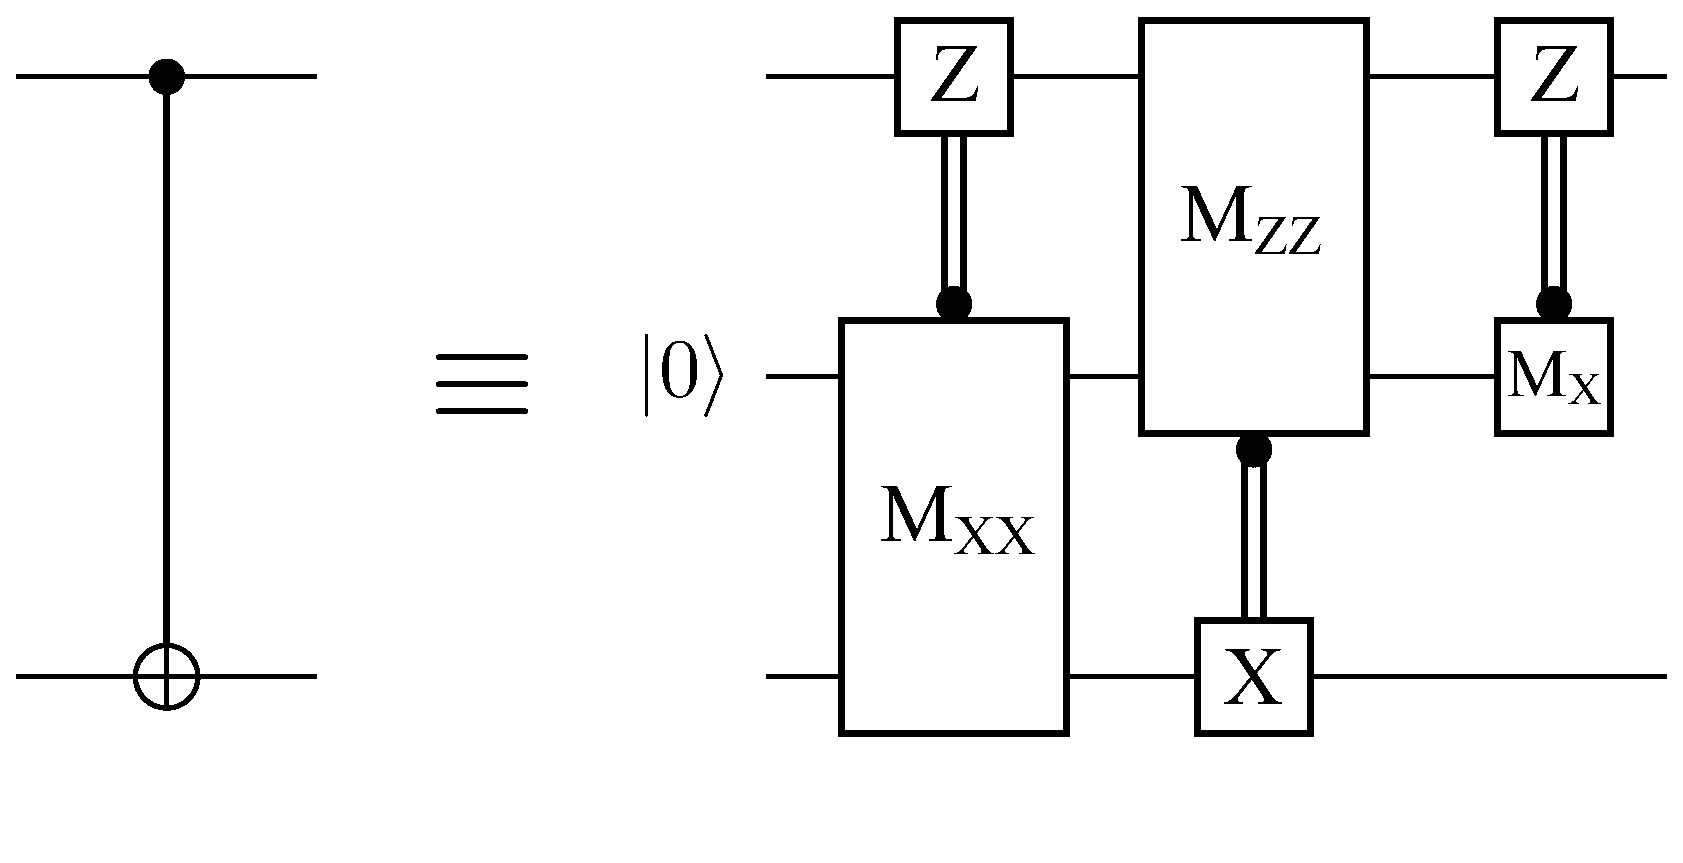
\includegraphics[scale=0.30]{figure/logical_cnot.eps}
            \vspace{0pt}\caption{}
            \label{logical_cnot}
            \vspace{-10pt}
        \end{figure}

        In the previous sections, we have seen the measurement operation $Z_1Z_2$ ($X_1X_2$) for logical qubits. Ignoring the Pauli correction based on the measurement results, as long as a 2-weight Pauli measurement on the logical qubits can be performed, we can achieve a CNOT gate.

        \begin{figure}[h]
            \centering
            \includegraphics[scale=0.25]{figure/cnot_in_lattice_surgery.eps}
            \vspace{0pt}\caption{}
            \label{cnot_in_lattice_surgery}
            \vspace{-10pt}
        \end{figure}


    }
}
\end{document}